\chapter{Methodology} \label{chapter-methodology}



\section{Resilience}

% There are two types of resilience questions when any system is shocked, does it return to an equilibrium state, the stability question, and does it return to the same kind of equilibrium---the hysteresis question. % We focus on the latter question.  

Historically low interest rates, and financial crises, have been a primary driver of rapid inflows of financial capital, accelerating the process, which raises the question of what will happen as interest rates rise. The analysis suggests however that there is hysteresis, that both the economic upswing and the downswing pull wealth out of communities, like a kind of ratchet or peristaltic pump. We analyze and model these dynamics in the resilience Chapter, %Chapter~\ref{chapter-resilience}

The model gives a resilience result which is that shared wealth through housing is not resilience.

It can also be used with a driven version of the model to show that the model pumps wealth out on the upswing and on the downswing - like a kind if ratchet.


\section{Resilience background}

This section explores the resilience dynamics of distribution of wealth within a class of market models.  

Using a systems design approach and looking at resilience measures and alternative regimes gives insights into patterns of distribution and how that shapes wealth. 

The two significant concepts of resilience for this work are the relationship between distinct alternative regimes and patterns of cycling within a single regime. 

\section{What is resilience and how is it connected to this work}

Resilience is a concept that has to with the way in which a system resists disturbance or maintains identity through disturbance. The concept has emerged independently with different, but related definitions in various fields. 
There are a class of systems that this idea of resilience should be applicable or illuminating for, however the concepts and measures that exist already are ill-suited to the dynamics of the system. 
The work in this thesis draws from the measures from existing measures and concepts of resilience from various discipline to evolve a measure that can apply to this other class of systems. 

Shaping this core broadly applicable concept that 
We can approach change in various systems using technical tools that are transferable. 
The concept 

\section{Resilience in engineering}

In engineering, Resilience is defined as the return properties of a system. 
It is the measures relating to how a system comes back to its stable equilibrium or stable state. For example if you push a branch on a tree, it will oscillate and settle back to its resting position. 

Stability properties are important in engineering because engineers are responsible for signing off the performance of system, whether the the system is a bridge or a chemical reactant or an electrical circuit. Stability is an aspect of the system's behaviour. The engineer needs measures to predict the stability of the system when it's perturbed. (Specific) 

Engineering resilience is distinct from the failure zones or the threshold of failure - for example the level of force/weight or number of stress cycles that would be required to collapse a bridge. While those measures pertain the thresholds beyond which the system would fail, resilience is about describing how the system recovers from perturbations that do not break it. 

The primary measure is how long the system takes to return to its equilibrium, i.e. the return time. (Equation) There are seven measures, listed in table XYZ that pertain to return to equilibrium properties.  (Table)

There is some variation in the use of the concept in specific disciplines of Engineering. For example, in transport engineering it has something to do with traffic flow.

\section{Resilience in ecology}

In Ecology resilience is defined as the way in which systems maintain identity through transformations. 

In engineering, the concept of resilience centres on the idea of a single equilibrium. If the system is not disturbed, it will stay at equilibrium and the resilience measures account for the system's return to this equilibrium. In the ecology, on the other hand, instead of a single equilibrium the underlying pattern of the system has a dynamic structure. For example the ecosystem of a forest contains ongoing cycles of life and death and evolving patterns and interactions and yet sustains its identity as a forest. 

An ecosystem can experience big shocks or disturbances without losing its basic identity. For example, there can be drought, floods, fire, species loss, etc and the forest can recover and continue to be a forest. (The forest can regrow, one species might replace another and the forest changes but it doesn't necessarily stop being a forest.) But some disturbances can tip the ecosystem over into a different pattern of functioning. For example if the land is cleared and animals come into to graze the seedling trees so that they do not grow back, the forest can transition to a grassland ecosystem. Or if the region becomes dry enough, the forest can transition to become a desert. 

In ecology these alternative patterns of a system that may be identified as a forest, grassland, or desert are called regimes. In Ecological resilience studies, this concept of regimes replaces the simpler idea of equilibrium, differing both because the underlying pattern is more complex and because there are multiple regimes that the ecosystem of the same land can shift between. 

Part of what resilience in ecology is getting at, then, is what kind and how big the disruption can be before the ecosystem becomes a different kind of ecosystem. Resilience measures describe the properties of these distinct regimes and the relations between them. The most common measure is the size of the perturbation the system can withstand without transitioning into an alternative pattern of functioning or regime.  

This approach to resilience was introduced by C.S. Holling with his 1973 paper on a Spruce Budworm model of a forest ecosystem. In this paper he argued that there was an evolving interrelationship/feedback cycle between Spruce growth/regrowth and the population of Spruce Budworms that eat them. This interaction drove ongoing cycles of forest recovery and collapse. 

Holling's work established the concept of these kinds of cycled and alternative regimes in ecosystems. Subsequent work by Marten Scheffer in lake eutrophication validated that alternative regimes appear in ecosystems in the real world. Now there is a database tracking thresholds and regime shifts in ecological systems with over a hundred entries showing its common.  ([https://www.resalliance.org/thresholds-db](https://www.resalliance.org/thresholds-db)) 

In ecology, this idea of resilience has evolved into a dynamic concept that is important in climate change science and ecological conservation. Resilience measures show how a system maintains identity through change by measuring the relationship between regimes, that is how close a system is to transitioning to a different regime or pattern of functioning. Thus the concept of ecological resilience and alternate regimes give tools to understand what is possible for an ecosystem. This give insight both into how ecosystems can be preserved but also what happens when they transform. 


\section{Resilience in social systems}

The ecological concept of Resilience has since been applied widely to various systems across disciplines (*INSERT EXAMPLES*). Frances Westley applies Holling's idea of alternative regimes to social systems as the basis for a theory of social innovation. 

Westley defines social innovation as ``a change in the routines, resource flows, authority flows or beliefs in any social system.'' According to Westley ``a successful social innovation also has durability and broad impact.'' 
Her studies in social innovation focus on how individuals, groups, or institutions are able to shift social systems to achieve certain goals. 

Westley's research question is how social systems transform. This frame differs from the majority of resilience work in engineering and ecology because the focus there tends to be on maintaining the integrity of the system, whereas Westley's work is focused on how to move between regimes. 

For example, in the Great Bear Rainforest in British Columbia in the late 1990's (??) clearcutting for pulp and paper was threatening some of the last old old growth forests in the region and disrupting the lives of people who depended on them. Over years of unchecked logging combined with a history of land appropriation, there was ongoing local resistance. In 199X images of the devastation spread through international media and led to a boycott of paper products from clearcutting. This moment of crisis brought the forestry industry to the table. After a carefully structured process of conversation and engagement between community organizers, political leaders, and industry they put the Great Bear Rainforest under Indigenous community control. 

This change in governance structure can be understood social system that can be understood as a regime change because there were a set of patterns and feedbacks holding the old system in place and and there new set of patterns and feedbacks holding the new system in place. Each regime has a distinct pattern of functioning or identity. 

The idea of resilience in social innovation illuminates how the patterns of different regimes structure the social systems. What is different about the two regime in the case of the Great Bear Rainforest is the distribution of the flow of money and power - or the the language of social innovation, resources and authority. This changed the routines and habits of the people making up the social system as they became more directly involved in managing the forest. The result is that the ancient Great Bear Rainforest survived. 

The study of resilience within social innovation looks at how actors within  systems play a role in shaping transformation of interconnected social-ecological systems. Westley specifically studies individuals, groups, or institutions who have the intention to shift social systems to achieve certain goals. This means that there is a directed strategic nature to the agents. This is illustrated by the case of the Great Bear Rainforest by the different stakeholders from industry, community and governance who are are all actively working to achieve specific goals. However none of these actors are outside outside the system. Even those with power cannot completely control the system. Their efforts interact with the actions of others and the broader context of the whole

Social systems are dynamic. There is no fixed equilibrium and yet they have clusters of properties that persist and can prove difficult to change. These patterns with distinct identities are described in social innovation theory as regimes. These patterns can pertain to various feature, from the routines that structure interactions to resource flows within the system. In the example of the Great Bear Rainforest, under the previous system the resources and money flowed out of the community and decisions were made by distant corporations. The shift in governance structurally affected both the ecosystem and the culture of the communities. When they shifted to community governance, the emphasis shifted away from extraction and toward investing and building the forest and the community. (ADD CONCRETE DETAILS/NUMBERS?) 

Sometimes people can achieve their goals and sometimes they do not and it depend on both what they do and the state of the system. In her grounded theory work studying people who have attempted and succeeded in changing systems, Westley observed that sometimes there are moments of opportunity that make shifts in the system possible.  In the rainforest example, there were years of Indigenous organizing and building an environmental movement. 
The change became possible at a particular moment when commodity prices were placing pressure on the industry and coordination between local and national environmentalists resulting in international boycotts of pulp and paper products from clearcut forest, particularly across Europe. The indigenous organizers were able to achieve more in this moment of opportunity.

According to Westley a successful social innovation also ``has durability and broad impact.'' This is a description of the change but it also illuminates how the resilience concept of regimes is useful. One feature of systems is that a set of feedback loops will hold patterns of interactions, resources flows, etc in place. Many changes simply die out.  The changes that last do so because they change the flows and dynamics in ways that are held in place by new feedback loops.  Social Innovation theorists have used the concept of regimes to explain this phenomena. If the system state is perturbed enough another set of patterns can come to dominate.  (MAKE SURE THESE TERMS ALIGN WITH THE PRECISE TERMINOLOGY USED LATER) In the example, after the shift to the community governance that became self-reinforcing as different feedback loops emerged to structure the building of relationships and institutional structures, community habits, networks of support, and resource flows. 

\section{Role of this thesis}

What has been articulated in Social innovation theory is a story of how feedback loops hold the patterns in place  and how systems can switch between sets of patterns. Westley and others have applied the concept of resilience as an explanatory framework, rather than as a a precise mathematical statement. 
The thesis seeks to operationalize these concepts within a formal model in the context of social systems. 


- By operationalizing into this model, we can patterns in how systems shift between regimes. Specifically in this thesis the models show where in the systems there are opportunities - ie the system is more vulnerable or -open to change. 
- In practice regimes change can move you into a more or less desired state. Here I focus on opportunities and interventions. 
- Inventions are \dots
- By looking at where the system has opportunity to change this work illuminates how actors might be able to identify opportunities for regime change. 
- 











he analysis has been applied conceptually, rather than as a precise mathematical statement. Thus far, in the study of social innovation 

Routines, resource authority flow and beliefs. 

International concern
Boycotts 
Political movement

Effective local movement established an indigenously led sustainable forest and tenure
It 



Community leaders were able to establish a 




Social innovation involves interventions or actions 




She studies I

Change in technology and demand for wood. 

For example, she looks at how various countries responded to the AIDS crisis and how activists in certain shaped 

There's a debate about how systems transform. 
Impersonal forces of history like the development of agriculture
She's studying the phenomena of change in order to inform 
The research is about how people try to change the word. 

(ie. a system consisting of different interconnected entities such as  individuals, groups, and institutions relating to each other and forming a whole.)

An interdependence of a social and cultural element 

Series of interrelationships between individuals and groups and institutions forming a whole. 



% [[adaptive cycle]]


\section{Resilience and class}

(TODO: introduce the idea of class in the resilience section, and link it to the resilience of the wealth trajectories.)  
reversibility/hysteresis, and how class is treated in the literature.
Three spatially segregated `classes.' Capitalists live in some spaceless utopia,  Urban workers who commute and earn wages in the urban commuter-shed, and  rural residents and landowners who may choose to move to the city. There may be a band surrounding the city or persons who do not commute but enjoy urban consumption amenities. 
a fourth class, the urban tenant. 
Developed in Chapter~\ref{chapter-model} on modelling.

The model is we employ consistent with the theories of Ricardo and Henry George in locating the ground of urban exploitation and class in the capacity to extract social surplus through land ownership, and differs from the standard Marxian analysis in its reliance on access to financial capital rather than control of productive physical capital. The paper concludes that given existing land ownership patterns which encourage speculative investment, housing prices must rise and income inequality must increase. 

In the classical language, someone is exploited if someone else gets a share of the value of their labour. %(REPLACE WITH MORE PRECISE DESCRIPTION). 
 Employers capture a share of the value of workers' labour, so they exploit workers under this definition.
Those who own land early in a growing city are also capture a share of everybody's production. Since they capture a share of the productivity of others working in the city, through the rents, they are also exploiters, they form a kind of hybrid class. %Rents could be captured directly through renting out the property after they retire away from the city,  or by selling the property at a higher value than they bought it. 


\section{Overview}

ANY OF THIS HERE?
Because of the gap, we had to bring together bunch of pieces, and the way we did that ended up being kind of methodological contribution \dots
Once we have this model it is useful for also understanding the wealth effects, in particular the resilience dynamics
Resilience is an under used concept in economic analysis for a few reasons. We show an example of that type of analysis based on hysteresis here. 

- a number of themes get in as bonus themes.

% Although many  who employ ABMs to analyse urban systems are deeply skeptical of neoclassical assumptions This demonstrates % in this context how %easily and productively 
 %, linking traditions that have been separate. 
In general, there is relatively little work rigorously linking analytic and agent based models, so the results can be understood formally, in relation. % incorporated into prior traditions and

***
DOC START

In this chapter we discuss the methodological approach of the thesis, as well as a number of modelling decisions. 


We are focused on the evolution of a city. In a city, people and organizations make individual decisions independently, constantly adjusting and shaping the city they inhabit. As a result, cities evolve continuously and and don't reach any final equilibrium. 
%In any city, numerous people and organizations in the city are making individual decisions independently, constantly adjusting in sensible ways to the changing parameters of the city they inhabit. As a result, cities evolve continuously and may never be in equilibrium.  To model this complex, dynamical, multi-agent economic system we  rely on techniques and insights from several fields and we  employ two distinct modeling approaches. We develop and explain the theoretical foundation of our work using a range of results from the economic  literature. We go on to implement the theoretical model in the agent-based modeling (ABM) framework. 
% In doing so we are attentive to the strengths and weaknesses of the approaches that we are adopting. 

\subsection{Equilibrium versus agent-based modeling}

Economists rely heavily on equilibrium analysis in their study of complex systems. 
%In Economic modelling the most familiar approach is the  analysis of systems in equilibrium. 
A set of necessary conditions describing a steady state of interest are imposed and then solved to find features of the equilibrium they generate. It is a productive methodology partly because it  bypasses the complex process of adjustment, focusing on the conditions that must be true if a particular situation is to persist.

The classic example is the ubiquitous supply and demand model. Each curve represents plausible behaviours of a class of agents. A situation is unlikely to persist if either class of agents is unsatisfied with the combination of price and quantity. The model explores the combinations that satisfy the behavoural intentions of both classes i.e. are on both curves. If the two curves can be described mathematically, equilibrium prices and quantities can be derived solving the two-equation system.

The approach produces tractable models that can often be solved explicitly. To achieve tractability, it is often convenient 
to limit the number of independent decision-makers by employing a ``representative agent.'' To extend the analysis to dynamic systems, ``laws of motion'' (adjustment rules) can be added in the form of either difference or differential equations.  Models quickly become intractable with more agents or dynamic 
processes, and economists, like other modellers, resort to simulation 
and numerical methods. 

In an \gls{ABM}, agents are defined as having adjustment rules or behaviours that respond to environmental variables.\footnote{This approach is not unfamiliar to economists - The Cournot duopoly model, for example, is analyzed using `reaction functions' which simply describe a firm's optimal response to as second firm's output choice.} 
Unlike equilibrium approaches, agent-based modelling commits to using computational methods to mimic the distributed decision making of complex systems like cities. A program is written that considers each agent sequentially and updates agent and system statuses as it goes. The program is allowed to iterate, and the values of any state variables of interest are recorded at each step. The model may or may not settle into a steady state. As with other modelling approaches, ABMs can be used explore the behaviour of the system by varying individual parameters, and to explore the parameter space using Monte Carlo methods.

% In ABMs it is often makes sense to simplify models, less for computational reasons then to % The problem of model complexity remains a challenge with ABMs, however, and modellers introduce simplifying assumptions. These are not as a rule needed for the computational model but are helpful in maintaining a focus on the key theme  of the model.  %(ADD distinction between detailed models and detailed explicit models)

We draw heavily on existing economic analysis of cities to identify relevant behaviours and parameters. We also employ three key economic equilibrium conditions drawn from the economic literature: a locational, labour market, and a housing market equilibrium conditions
%Some adjustments are slow and some are fast. Rates of adjustment can matter. 

Because our focus is financialization in the land market, we use the equilibrium conditions for competitive labour markets to bypass the complex and partially understood wage-setting process. We assume, a core theoretical result from the theory of the firm, that workers are paid their \gls{marginal value-product}. We ground this approach in recent research that has derived and estimated an aggregate urban production function consistent with modern \gls{neoclassical growth theory}.\footnote{We are not aware of other research that has taken this step yet.} We use the result to derive an urban wage premium that drives city growth. We would argue that, since housing and labour markets can adjust more quickly than urban productivity, we can assume that they respond  continuously to the slower movement of population and productivity. % need to reference? 

A similar market-based argument allows us to assume that land rents are determined by the classic urban locational equilibrium. The theory is based on the insight that if individual utilities are higher at one location in the city, entrants or movers will choose that  location. This is an implication of consumer choice theory. In a market with any degree of churn market prices for land should converge on use values, and these will vary systematically with transportation costs. For simplicity, we present the model for the case where individuals have the same preferences, employment opportunities and transportation costs. Building on this, %In the computational model 
we can introduce site-specific and person-specific features. 

ALTERNATE PHRASING? Transportation costs depend on distance from the center, so land close to the center is more attractive than land farther away.  The equilibrium concept is that a market with identical individuals with identical incomes and transportation costs will result in identical utilities. The result is that land rent must decline with distance from the central place to offset rising transportation cost. 

Finally, we employ \gls{equilibrium reasoning} in the housing and investment process. We assume investors behave rationally in that they estimate the potential returns on their investments and seek the highest returns they can get. They calculate an offer price in each transaction based on several factors: land rents, expected price changes, their individual price of capital and discounting rate, and the information available to them.

It is at this point we introduce an innovation to formal urban modelling. We draw on the literature for the relevant `\gls{stylized facts}' about differences in these values based on wealth and income. This opens the possibility of urban segregation and the endogenous emergence of \gls{class} distinction based on capital access, a process explored by John Roemer in his neglected General Theory of Exploitation and Class \cite{roemerGeneralTheoryExploitation1982}.  

\Gls{expectations} have to take into account some amount of current and past information. Forecasts based on recent price movements can give rise to \gls{price bubble}s through either speculative or precautionary motives. Expectations anchored in \gls{perfect foresight} have different dynamics, since agents correctly forecast the path of prices \cite{muthRationalExpectationsTheory1961}. We employ backwards-looking expectation formation anchored 
%  This ANCHORING IS INTERESTING, BY THE WAY
to current rental returns, which allows agents to be misled by rapidly rising prices. We derive an investment rule of this sort in Chapter~\ref{chapter-financialization}. 

\subsubsection{SORT - single value frontier - explore reasons}
WHERE TO EXPAND% *** We will explain why  the rent charged to the tenant is locked  to a single value. A few factors - we are looking at the frontiers- the economically justified maximum as a way of linking productivity and extraction formally. - there are many variations and extensions to build on/explore/relax these core assumptions - - want to do this for a few reasons \dots

(MAYBE ADD THIS? Note: we do not assume equilibrium conditions in the agent model, however our approach is to stay close to the analytic tradition, relaxing assumptions to clarify what drives each results, and connect the work with classical and neo-classical theory \dots)

\subsection{Overlapping generations}
In our model individuals have a working life, then retire. If they own homes they sell and move to the countryside where housing is cheaper. They are replaced by new entrants from the countryside. New entrants may become buyers or tenants. This is a variant of the \gls{overlapping generations}  model in which savings are passed on to the next generation. In our case homes are passed on, as agents retire and move away. While the model has multiple generations, it is not a `dynastic' model in which the generations are linked by family ties and inheritance matters in individual decision-making. We rely on this simple version because the core issues for us are  the effect of financialization on city productivity, whether the city continues to provide opportunity for newcomers and those without the benefit of generational wealth and the emergence of classes. Introducing a richer family structure would complicate the model but add little to understanding  our  main  issue. 

\subsection{Urban and rural wages}
A modelling device that plays a major role is our use of the \gls{urban wage premium}, the difference between a rural and an urban wage driven by positive \gls{agglomeration effect}s on productivity in the city. It cannot be competed away because transportation costs limit access to the productive centre. The wage premium is a partial measure of the agglomeration effect. It generates the \gls{rent premium} on urban land. In this thesis we want to call attention to the distribution of that rent premium.

To simplify the analysis, we assume that we can partition actual wages between the wage premium,  and all other expenses. The wage premium  is available for accumulation or to be spent on transportation. We assume both urban and non-urban populations  receive a \gls{subsistence wage} which covers  the cost of buildings, food and other living costs and a base cost of land. This analytical device appears in classical models (Malthus, Ricardo, Marx) as a subsistence wage. In most urban models it is described as the cost of agricultural land, or more precisely,  as the opportunity cost of urban land at the margin. We simply extended the technique to combine the opportunity cost of urban labour and land, allowing us to focus on the rents themselves. 


There are advantages and disadvantages to this technique. The motivating advantage is that it lets us isolate the social surplus generate by agglomeration. One disadvantage is that it suppresses many issues that are of interest in other contexts - such as choice of home size and quality. In the computational model it is easy to allow for different building types and more complex housing choice, but in this section we simply  want to make the logic of our model as clear as possible. We foresee adding layers to the computational model that incorporate redevelopment and construction and allow for decisions about scale, type and location. 

Another disadvantage of technique in the analytical version is that it does not allow us to make speculation on  the value of  buildings part visible. It is a problem that is dealt with in the computation model, but we believe the added complexity will not add clarity here. Research (see \cite{mcdonaldWilliamAlonsoRichard2007}) has shown  that the core model is robust to many extension of this sort. 

\subsection{Income, wealth and savings}
\begin{verbatim}\color{red}



savings = 0 # = working_age*savings_rate*psi + savings_rate*(omega-c*d) #second part  only if owner 
            # everyone saves out of subsistence and owners save out of economic rent 
            # lifetime income of owners diverges from rentors even though current income does not. 
            # this matters if they buy  a rental property, otherwise it disappears into current consumption and retirement standard of livineg
            # relationship  between income and consumption is suppressed by forcing a uniform subsistence wage.

QUESTION - SHOULD PART OF THIS DISCUSSION GO IN THE MODEL SECTION?
\end{verbatim}



\subsubsection{Examples of  \gls{equilibrium reasoning} in our analysis}

As an example of \gls{equilibrium reasoning},  we implicitly impose the locational equilibrium condition,
\[U_i(d,\dots)=U_j(d, \dots),\]where $U_i(d,\dots)$ represents agent $i$'s utility at distance $d$. 
The condition says that identical individuals must get the same utility no matter how far they live from the city centre. If that were not the case, individuals would move to a location where they get higher utility. For utility to remain constant as  transportation costs  rise, some other variable must compensate. In this class of models, rent charged for the use of land must fall as distance increases. Equilibrium locational choice by commuters therefore determines the extent and ultimately  population of the city.\footnote{More complex models allow home sizes and lot sizes in the suburbs to increase as well.} Since land value  is \gls{capitalize}d rent, land values also decline toward the edge of the city until they are equal to the rural value of land. 
% different location would take a long time to work through the system. Prices, however, can adjust much more quickly. 

An adjustment process that requires people to move to a different location would take a long time to work through the system. Prices, however, can adjust much more quickly.



%  It follows that 
% \[\frac{\partial U_i(d, d(dots)}{\partial t}=\frac{\partial U_j(d, /dots)}{\partial t}\]

We also rely on equilibrium arguments in our model to ``black box'' the productions sector and most of  the labour market, including most decisions by producers and wage demands by workers. 


\subsubsection{\Gls{marginal} vs \gls{inframarginal} quantities}
In relying on these equilibrium conditions, we are implicitly applying standard neoclassical economic methods despite the fact that our focus is not on the \gls{marginal} conditions that determine prices, but on the \gls{inframarginal} quantities that make up rents. We can illustrate with a diagram that is more fully explained in Chapters~\ref{chapter-rent} and \ref{chapter-space}. 

\begin{figure}[h!t!]
\centering
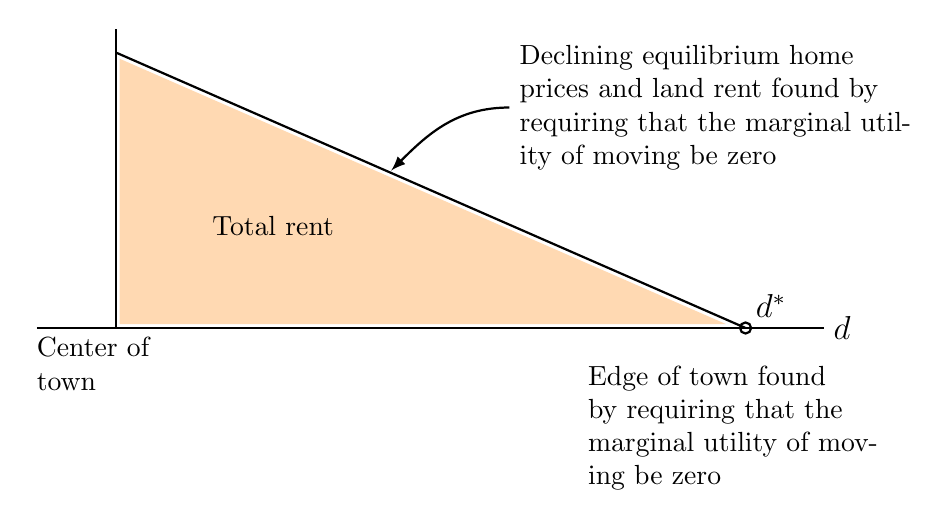
\begin{tikzpicture}[domain=0:2]
%\draw[thick,color=gray,step=.5cm, dashed] (-0.5,-.5) grid (3,3);
\draw[line width=.01] (0,0) -- (10,0) node[right] {\large $d$};
\node at (1,0) [below,text width=2cm] {Center of town};
%\draw[thick ] (0,3)node[above right] {merchant's price in town} -- (10,3) ;
\draw[thick ] (0,0)  -- (10,0); 
\draw[thick, -latex] (6,2.8)
node[right, text width=5cm]{Declining equilibrium  home prices and land rent found by requiring that the marginal utility of moving be zero} 
to [out=180, in=45](4.5,2); 

\fill[orange!30] (1.05,0.05)--(8.75,0.05)--(1.05,3.42)--cycle;

\draw[thick ] (1,0) -- (1,3.8);
\draw[thick ] (9,0)node [above right]{\large $d^*$}circle[radius=2pt] node[below=.35cm,text width=4cm] {Edge of town found by requiring that the marginal utility of moving be zero} -- (1,3.5) ;

\node at (3,1.3){Total rent};
\end{tikzpicture} 
\caption{Illustrating marginal and infra-marginal quantities with the bid-rent curve and aggregate rent.}
\label{fig-land-rent-as-inframarginal}
\end{figure}


In Figure~\ref{fig-land-rent-as-inframarginal}, The level of rent is determined at any distance by individuals making comparison locally. At point $d^*$ the person at the edge of the city decides whether to work in the centre or in the non-urban space. These are \gls{marginal} decisions. The orange area represents  the total rents generated between $d=0$ and $d=d^*$. It is a summation of \textbf{\gls{inframarginal}} rents. Like Ricardo in his classic study \cite{ricardoEssayInfluenceLow1815}, we are concerned with the distribution of rents, which are an  inframaginal quantity.


\section{Is it engineering?}

Engineering is the application of knowledge for safety. 

% Done very well, always emerged after crisis - holes in boars- stess corners, bridges fell. the regulatory structures got built in large part after disasters happened.

There's a class of dangers.
Class of disasters, climate - forest figher
neirbhourhodos burnign down, communtiies folled because of carbon

different because they are much more intertwined with human lives and hcoices on a day 
and whole system governance challenges.

Engineering
because it's not a narrowly constrained problem that can be governed at the level of controlling a design which can be released into the world. 

IT is much more intertwined.
Following attempts at social control
experiments in social engineering

The science of complex systems


And more generally the principles of how to promise offer a path forward. 

Resilience is not about state, its about regimes, it can be about about how to protect as much choice as possible.

Resilience is a principle we put here in methodology. 




- a bubble around the human, don't hurt it.
the risks now are systemic risks.
climate

science is centered on experimentation.


engineering has little place for resilienc.e

and control
Engineering combines 
complex systems

Nobody wants control theory, or reductionist science controling their state. 



% providing tractable models.  equilibrium analysis of marginal effects, and representative agents which hid distributional effects, as well as spaceless economic models of markets made it difficult to capture the richer spacial dynamics of urban rents, and the details of the ways economic forces play out for individual actors.

% First they've not tended to build in, in a sophisticated way classical economic theory,
% In general, classical economic theory has not been developed in agent-based modeling work
% Agent-based models have begun with simple models, using and relaxing neoclassical assumptions, and building from first principles. This is absolutely the place to start. As the field matures, it makes sense to introduce theory in a more nuanced way, that connects with classical theory/the history of thought, etc

% Second, relatively little agent-based modelling work integrates with the neoclassical economic work in a way that makes the relation clear/holds the advantages. ABM work tends to both reject neoclassical approaches and rely on neoclassical assumptions.
% More generally only a few agent models (e.g. spruce budworm) connect the analytic and agent models in a clear rigorous way. We focus on holding in addition to the relation with classical theory, a close connection with the many advances made withing neoclassical modelling

% - this connection will make it easier to incorporate in teaching and for mainstream economists to engage on and build with.

% This work builds, first, a simple conceptually clear model tightly integrated with the core economic modelling traditions, that builds on the theory of rent.

% ALSO (Agent modelling also tents to model individuals- we also take some steps to agent-based modelling beyond the individual, and to the work developing model in a mode ideas)

% Third, econ lacks resilience analysis and models, yet hysteresis clearly present in the relation between the built environment and econ activity. Although there's been work on dynamics and individual effects, there has been little work looking at the resilience dynamics in economic models, we take that approach looking at the resilience of community and individual wealth, and the relationship between that wealth and productivity. 

% - This puts resilience dynamics at the center of economic analysis.

% The resilience analysis looks at the dynamics of rent in economic boom and bust cycles.
% There is a ratchet effect, achieved through hysteresis in the system, in which sucks wealth out of communities on the way up and on the way down. % DETAIL ONCE DRAFTED.


% \section{Other notes - to sort}

% % TEMP - here are some other notes we may want to reference or bring in. [[non individualistic modeling of agents]] [[generalizability in agent vs classical econ models]]

% The emphasis is on clarity and connecting with the equilibrium in economics, and systematically relaxing each, to connect with the analytic tradition of economic modelling
% The clarity of intuition of the neoclassical tradition with the deeper root of distribution theory rooted in classical economics and the breath and rigor possible with new tools from the study of complexity and statistical physics.

% Methodological questions: 

%     - agent models (integrating theory more completely into agent models)
    
%     - rent theory

% Core model

%     - static version
    
%     - dynamic version

% Simulations
% Result - hysteresis,
% Policy





% TODO Rename file/label as an appendix, or fill out and make into a chapter again
% In addition to the core contribution linking housing and productivity, there are three methodological lines of contribution, and there are policy implications SUMMARIZE METHODOLOGICAL CONTRIBUTIONS %(rent is key to financialization, however the main urban models don't observe the distribution of rents)


% \subsection{Systems design engineering and the systems level effects of financialization}
% Appropriate for systems design engineering
% - engineering is science to responsibility.

% \section{Political economy}

% early stocks, company run an army to take over land and claim surplus in India- more in line with military/state conquests
% then that translates into the industrial economy
% the notion that productivity came from industrial productivity or human capacity.

% what's question, what went before - politics and economics. department of political economy into the 1960s- politics and older ideas.

% Coarse graining, the scale problem.
% Cross scale modelling, models as library components, fall down and rise up wiwth scales
% Building blocks as toys to play and think with - simple enough assumptions to build with








% \textbf{the french engineers} - method math and back \dots

% econ a kind of reactionary precursor to complex systems.  Adam smith- methodological evolution. ABM and link model.

% not an exercise in modelling, it's an exercise in understanding what's happening
% want to know what's happening in society and what we can do. why we want to talk about hysteresis and the effects on social classes.

% haven't formulated even the theoretical model
% rent and social class not in the alonzo model
% couldn't track whose in what class when you do your analysis of scaling
% large gap but hard to see since not maped, theoretical objects barely formulated.

% DISCOVERY PROCESS
% An accident that we found this model, looking for someone to have answered this, planned to just use economic theory.

% thought the model \dots 

% - to move with the dynamism of how people think. 

% (personal ethnography, co-creation, activist method from australi.)

% Simple agent based modes
% TO DO THIS -
% having done this rockefeller work-- wanted to move between omdels way people thing.

% core decsions fast \dots
% get good results and hold core details in their head \dots

% lots of great models out there. 

% \textbf{Coarse graining, curse of dimensionality}
% flow between these classes of models.

% WE DO THIS
% Link agent based and analytic models.

% conceputally clear modelling traditon not connected to one that lets you look at individual trajectoreis---

% - distribution, a farm, unemployed youth \dots bring in infrastructure from well defined simplified models

% abm is in some ways simpler- this agent does this. 
% -- get input asking someone questions- this is wha t people knwo - do this as a buyer \dots ive assempled these piece \dots

% (we've made it a well formed question by making it a model structure. accepted the conventional knowlege about he large scale dynamics \dots
% formulated the conventional knowleges so it can talk to the input \dots )


% -wasn't clear why we couldn't get what we needed from econ.
% did a bunch of work building a biger model, lots of discusion about the \gls{transmission mechanism}.
% We realized it shoudl be coarse grained. 

% REPRHASE METHODOLOGICAL CONNTRIBUTIONS FROM INTRO

% A MEANS IS USE OF THE 
% Constructing an urban \gls{agent-based model} that is consistent with {neoclassical growth theory}. We show how the neoclassical framework can be implemented in the agent-based framework, and make a case for the usefulness of the approach in linking urban rents and productivity. %Chapter~\ref{chapter-methodology} discuses methodological implications of this approach.

% THIS HAS IMPLICATIONS
% Building a model that is easily extended to explore a range of issues, and used to evaluate policy options. 
% The model combines clear and explicit theoretical assumptions with careful and transparent implementation of the logic. % in code \dots %flexible Python code.
%     % \item Providing a model that we believe
% We have taken care to allow for  both theoretical and policy-relevant extensions in the simulation,  building a base model that aims to be as simple as something like Alonzo's urban model \cite{alonsoLocationLandUse1964}, but 
% % To be useful in policy discussions, a model must  
% simulates the relevant system features and can incorporate a range of intervention types. %way the simulation model is coded. 


% IT LETS YOU DO THINGS THAT HAVE BEEN HARD
% - e.g. have tractible models that let you explore \textbf{hysteresis, reversibility}- hopefully bringing it towards the core of analysis
% Resilience.

% DOING THIS IN AN ENGINEERING DEPARTMENT
% Engineering  knowledge for responsibility - just like a bridge, a social choice to have a middle class.
% have housing for everyone, have food for everyone

% social engineering has been a sensitive point- efforts have tended to control.
% Particularly after WWII social experiments, that were horors.

% even building predictive modes is a problem. any intervention that makes your model predictive increases your control.

% Reductionism had some holdouts but largely unchallenged

% %Challenges to reductionism deep within the field too

% Answer is of course to relinquish commitment to state. 

% - syxtems and resilience give  a bridge
% What is the systems compenent - design for the properties- 
% clearly a system

% social engineering- a note on the approach to engineering in social system
% cannot know much about state- have to comite to regime, it is then possible to comit to things like freedom \dots
% to autonomy, relinquish comitent to stat


% RESILIENCE IS CENTRAL TO THE ADVANCE - TO ACTUALLY MAKING AN ENGINEERING OF THE SOCIAL POSSIBLE.


% at the level of capturing and sharing details.

% applied work
%

% has to do with Social innovation, how societies are transformed,
% gives an ease in relating the model with the action. 

% action and choice
% weak links in hosting, 

% did these models for rockefeller, for the labes-- had a group
% worked iwith the games intstitued ith design \dots
